% Asset ID: FA22TDistributionTikZ-001
% Source: Phase 1 lesson, Core Theory and Exam Technique Notes
% Related lesson section: # 9.5 Critical-region sketch
% Used placeholder: [VISUAL PLACEHOLDER: FA22TDistributionTikZ-001 | Source: Core hypothesis-test method | Insert from tikz/FA22TDistributionTikZ-001.tex | Purpose: Show one-tailed and two-tailed t-test critical regions.]
% Purpose: Show left-tailed, right-tailed and two-tailed t-test critical regions, including observed t-value markers and reject/do-not-reject decisions.

\documentclass[tikz,border=8pt]{standalone}
\usepackage{amsmath}
\usepackage{xcolor}
\usetikzlibrary{arrows.meta,positioning,calc}
\definecolor{Canvas}{HTML}{FAF9F6}
\definecolor{Ivory}{HTML}{FFFFF0}
\definecolor{LineSoft}{HTML}{E5E5EA}
\definecolor{Gold}{HTML}{C5A059}
\definecolor{GoldBright}{HTML}{D4AF37}
\definecolor{PinkSoft}{HTML}{FBEFEF}
\definecolor{TextDark}{HTML}{2C2C2E}
\begin{document}
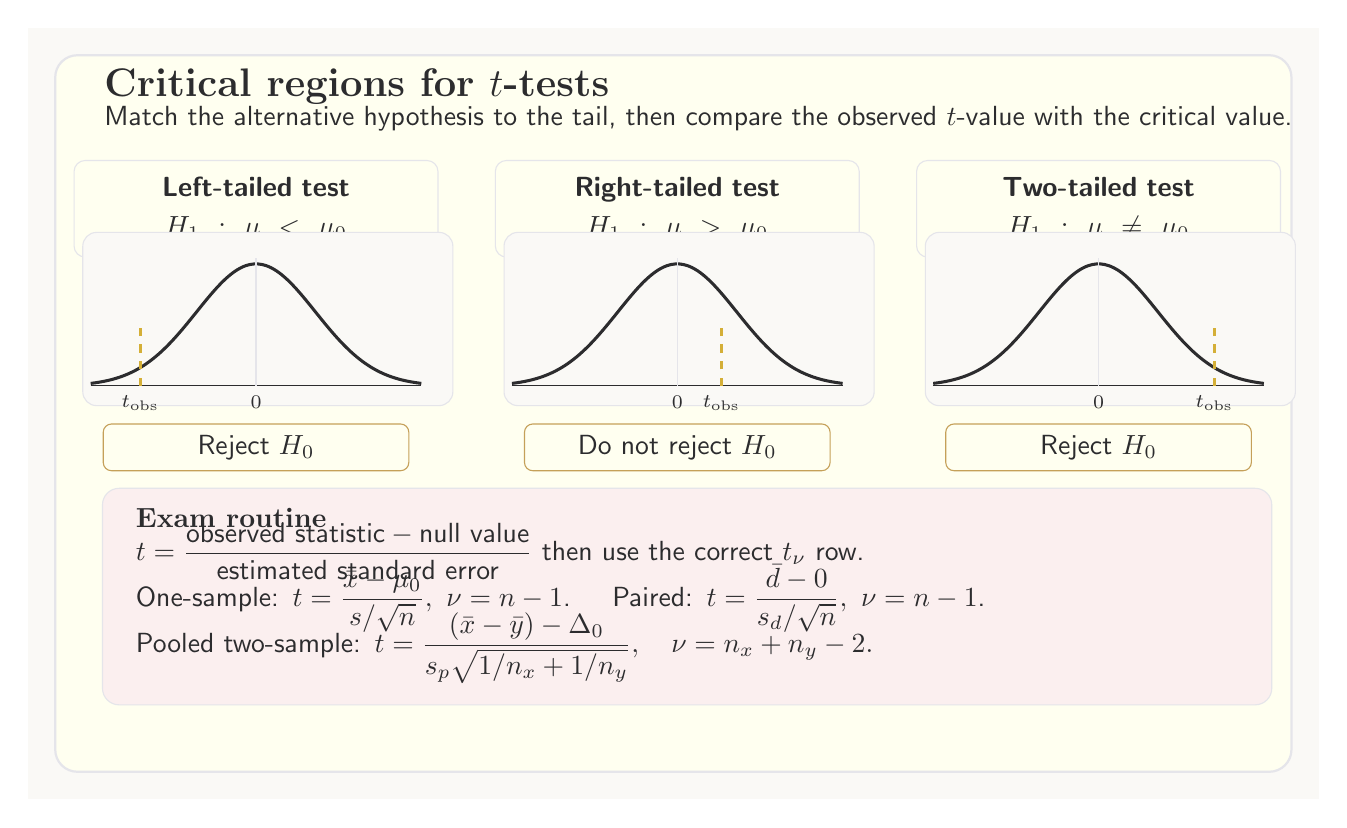
\begin{tikzpicture}[font=\sffamily,text=TextDark,>=Latex]
\fill[Canvas] (-0.8,-1.1) rectangle (15.6,8.7);
\draw[LineSoft,line width=0.8pt,rounded corners=8pt,fill=Ivory] (-0.45,-0.75) rectangle (15.25,8.35);
\node[anchor=west,font=\bfseries\Large] at (0.05,7.95){Critical regions for \(t\)-tests};
\node[anchor=west] at (0.05,7.55){Match the alternative hypothesis to the tail, then compare the observed \(t\)-value with the critical value.};
\foreach \xshift/\title/\alt/\shade/\obs/\decision in {0/{Left-tailed test}/{H_1:\mu<\mu_0}/left/-2.1/{Reject \(H_0\)},5.35/{Right-tailed test}/{H_1:\mu>\mu_0}/right/0.8/{Do not reject \(H_0\)},10.7/{Two-tailed test}/{H_1:\mu\ne\mu_0}/two/2.1/{Reject \(H_0\)}}{
\begin{scope}[shift={(\xshift,4.15)}]
\node[rounded corners=4pt,draw=LineSoft,fill=Ivory,inner sep=6pt,align=center,text width=4.2cm] at (2.1,2.25){\textbf{\title}\\[2pt]\(\alt\)};
\draw[LineSoft,rounded corners=5pt,fill=Canvas] (-0.1,-0.25) rectangle (4.6,1.95);
\ifx\shade\left
\fill[PinkSoft] plot[domain=-3:-1.4,smooth,samples=50] ({2.1+0.7*\x},{1.55*exp(-0.43*\x*\x)}) -- ({2.1+0.7*(-1.4)},0) -- ({2.1+0.7*(-3)},0) -- cycle;
\fi
\ifx\shade\right
\fill[PinkSoft] plot[domain=1.4:3,smooth,samples=50] ({2.1+0.7*\x},{1.55*exp(-0.43*\x*\x)}) -- ({2.1+0.7*(3)},0) -- ({2.1+0.7*(1.4)},0) -- cycle;
\fi
\ifx\shade\two
\fill[PinkSoft] plot[domain=-3:-1.6,smooth,samples=50] ({2.1+0.7*\x},{1.55*exp(-0.43*\x*\x)}) -- ({2.1+0.7*(-1.6)},0) -- ({2.1+0.7*(-3)},0) -- cycle;
\fill[PinkSoft] plot[domain=1.6:3,smooth,samples=50] ({2.1+0.7*\x},{1.55*exp(-0.43*\x*\x)}) -- ({2.1+0.7*(3)},0) -- ({2.1+0.7*(1.6)},0) -- cycle;
\fi
\draw[TextDark,line width=1.1pt,smooth,samples=80] plot[domain=-3:3] ({2.1+0.7*\x},{1.55*exp(-0.43*\x*\x)});
\draw[TextDark] (0,0) -- (4.2,0); \draw[LineSoft] (2.1,0) -- (2.1,1.62);
\draw[GoldBright,line width=1.1pt,dashed] ({2.1+0.7*(\obs)},0) -- ({2.1+0.7*(\obs)},0.8);
\node[below,font=\scriptsize] at ({2.1+0.7*(\obs)},0){\(t_{\text{obs}}\)};
\node[below,font=\scriptsize] at (2.1,0){0};
\node[rounded corners=3pt,draw=Gold,fill=Ivory,inner sep=4pt,align=center,text width=3.6cm] at (2.1,-0.78){\decision};
\end{scope}}
\draw[LineSoft,rounded corners=6pt,fill=PinkSoft] (0.15,0.1) rectangle (15.0,2.85);
\node[anchor=west,font=\bfseries] at (0.45,2.48){Exam routine};
\node[anchor=west,align=left,text width=14.1cm] at (0.45,2.05){\(\displaystyle t=\frac{\text{observed statistic}-\text{null value}}{\text{estimated standard error}}\) then use the correct \(t_\nu\) row.};
\node[anchor=west,align=left,text width=14.1cm] at (0.45,1.45){One-sample: \(\displaystyle t=\frac{\bar{x}-\mu_0}{s/\sqrt n},\ \nu=n-1\). \quad Paired: \(\displaystyle t=\frac{\bar{d}-0}{s_d/\sqrt n},\ \nu=n-1\).};
\node[anchor=west,align=left,text width=14.1cm] at (0.45,0.82){Pooled two-sample: \(\displaystyle t=\frac{(\bar{x}-\bar{y})-\Delta_0}{s_p\sqrt{1/n_x+1/n_y}},\quad \nu=n_x+n_y-2.\)};
\end{tikzpicture}
\end{document}
